\documentclass{article}
% Useful packages
\usepackage{amsmath} % Required for advanced math typesetting
\usepackage{graphicx} % Required for inserting images
\usepackage{xcolor} % Required for color definitions
\usepackage{listings}
\usepackage{tcolorbox} % Required for creating boxes
\usepackage{float} % Required for controlling the position of images


% Code settings
\lstset{
    language=C,
    basicstyle=\ttfamily\small,
    keywordstyle=\color{blue},
    commentstyle=\color{green!50!black},
    stringstyle=\color{orange},
    showstringspaces=false,
    breaklines=true,
    frame=single,
    numbers=left,
    numberstyle=\tiny,
    stepnumber=1
}

\setlength{\parindent}{0pt}

\title{SEAI\_2024\_R12}
\author{Giulio Capecchi, Jacopo Niccolai}
\date{December 2024}


\begin{document}

\maketitle

\vspace{3cm}
\begin{figure}[H]
    \centering
    
\includegraphics[width=0.6\textwidth]{assets/unipi.png}
    \label{fig:unipi_logo}
\end{figure}

\newpage

\tableofcontents

\newpage

\section{Introduction}
This project focuses on the synthesis of the forward pass for three types of neural network architectures: a \textbf{Multilayer Perceptron (MLP)}, a \textbf{Convolutional Neural Network (ConvNet)}, and a \textbf{Transformer}, implemented on an FPGA (Field Programmable Gate Array).  
To achieve this, the network parameters were first obtained using Python and the \textit{PyTorch} library. These parameters were subsequently hardcoded into \texttt{C} code, enabling the hardware synthesis process.


\begin{figure}[H]
    \centering
    
\includegraphics[width=0.5\textwidth]{assets/vitis-hls.png}
    \caption{Xilinx Vitis HLS}
    \label{fig:vitis_hls}
\end{figure}

\textbf{Vitis Unified Software Platform} is a comprehensive suite designed to accelerate the development of applications on FPGAs, Adaptive SoCs, and ACAPs (Adaptive Compute Acceleration Platforms). By combining high-level software programming techniques with hardware-optimized implementations, Vitis enables developers to write applications in \textit{C}, \textit{C++}, or \textit{OpenCL} while leveraging hardware-specific optimizations for enhanced performance.  

In this project, Vitis plays a pivotal role in synthesizing the neural network architectures—MLP, ConvNet, and Transformer—onto the FPGA. Its \textbf{High-Level Synthesis (HLS)} tools allow for rapid prototyping and optimization of the \textit{C} code, ensuring efficient resource utilization, parallelism, and low-latency execution. The platform's ability to integrate high-level design, simulation, and hardware synthesis streamlines the workflow, bridging the gap between software and hardware development.


\section{Project Description}
\subsection{Workflow Overview}
The neural networks were constructed and trained using the \textit{PyTorch} library. Once trained, the weights and biases were exported to be hardcoded into the corresponding \texttt{C} implementation. The \texttt{C} code was specifically designed to be compatible with FPGA synthesis tools, such as Vitis HLS, ensuring efficient hardware synthesis.


\subsection{C Implementation}
The \texttt{C} code developed includes the forward pass for:
\begin{itemize}
    \item \textbf{MLP}: implementation of propagation through dense layers.
    \item \textbf{ConvNet}: handling of convolution and pooling operations.
    \item \textbf{Transformer}: managing complex operations like attention.
\end{itemize}

To optimize the C implementation for hardware synthesis, specific \textbf{HLS directives} were applied to critical portions of the code. These directives guide the High-Level Synthesis (HLS) tool to produce more efficient hardware designs by controlling resource allocation, loop unrolling, and pipeline creation. The two main directives used in this project are:

\begin{itemize}
    \item \textbf{\texttt{HLS INLINE}}: This directive forces the complete insertion of the body of a function or loop directly at the point where it is called, eliminating the overhead associated with function calls or separate hardware resource allocation. By doing so, it reduces latency by eliminating function call delays. However, it may increase hardware area usage since the logic is replicated wherever the function is called. It is typically used for simple or frequently invoked functions to reduce latency.
    
    \item \textbf{\texttt{HLS PIPELINE}}: This directive breaks a loop or function into multiple stages (pipeline), allowing multiple iterations or operations to execute simultaneously, thereby increasing the design's throughput. It enables processing of new iterations in every clock cycle (or at specific intervals called \textit{Initiation Interval (II)}). The options for this directive include \texttt{II=N} (to specify the interval between iterations, such as 1 clock cycle) and \texttt{rewind} (to automatically restart the loop after completion). It is typically used in loops that process large amounts of data to maximize throughput in repetitive operations.
\end{itemize}

These directives were applied strategically to balance trade-offs between latency, resource utilization, and overall performance. For example, \texttt{HLS INLINE} was used in frequently called small functions to minimize latency, while \texttt{HLS PIPELINE} was applied to loops processing neural network layers to maximize parallelism and throughput. The appropriate use of these directives is crucial for achieving efficient FPGA-based implementations.\\\\
It is important to note that the directives discussed in this section represent only a subset of the directives executed by the HLS compiler during the synthesis process. These directives were explicitly added to address specific warnings and improve the design's performance. They were carefully placed at the exact lines of code where they were required to resolve issues or optimize critical sections of the implementation.\\\\

\newpage
\textbf{Hardcoding Network Parameters}

The network parameters (weights and biases) exported from the trained PyTorch model were directly integrated into the \textit{C} implementation in a hardcoded manner. This process ensures that the FPGA hardware has direct access to pre-trained values during the forward pass, avoiding the need for external memory accesses and thereby reducing latency.

The specific details of how the weights and biases were exported, including the Python code used to save them into a text file, can be found in Section 4.2.3 TODO(check the correct section number). These parameters were then structured in the \texttt{C} code as arrays within the MLP structure, as defined in Section 4.3.1 TODO(check the correct section number). This approach, while limiting the flexibility of re-training or updating the model without recompilation, was chosen to optimize execution time and reduce complexity in hardware synthesis.


\section{Code Architecture}
\subsection{C File Structure}
The forward pass is implemented using a sequence of functions for each layer type:
\begin{itemize}
    \item Activation functions (\texttt{relu}, \texttt{softmax}, etc.).
    \item Functions for convolution and pooling operations.
    \item Functions for attention mechanisms in Transformers.
\end{itemize}


\subsection{Hardware Synthesis}
The code was designed to be compatible with tools such as Vitis HLS, leveraging specific pragmas to optimize the implementation.

\section{Multi-Layer Perceptron}
Let's analyze the implementation of the forward pass for a Multi-Layer Perceptron. The forward pass for an MLP consists of propagating the input through a series of dense layers, each followed by an activation function.
The code for it can be found inside the \texttt{PyTorch} folder, that contains the notebooks used to train the models and export their parameters.

\subsection{Dataset}
The MLP was trained using the well-known \textit{Iris} dataset, which contains 150 samples of iris flowers, each with four features and a class label (the last value of each row).
There is a total of three classes: \textit{setosa}, \textit{versicolor}, and \textit{virginica}.
The dataset was split into training and test sets, with 80\% of the samples used for training and 20\% for testing.

An example of the dataset is shown below:

\begin{tcolorbox}[colback=gray!5, colframe=black, rounded corners, boxrule=0.1mm]
\textbf{\textcolor{blue}{sepal\_length,sepal\_width,petal\_length,petal\_width,species}} \\
5.1,3.5,1.4,0.2,setosa \\
5.7,2.8,4.5,1.3,versicolor \\
6.1,2.6,5.6,1.4,virginica \\
...
\end{tcolorbox}

The dataset's labels were encoded as integers using the Scikit-learn \texttt{LabelEncoder} class, which maps each class to a unique integer value.
To facilitate its further usage inside the \texttt{C} implementation, this encoded version of the dataset was saved to a txt file, \textit{iris\_dataset\_encoded.txt}.

\subsection{PyTorch Model}
\subsubsection{Model Architecture}
The architecture of the MLP model consists of three fully connected (dense) layers.
The input layer has 4 neurons corresponding to the 4 features of the Iris dataset. 
The first and second hidden layers each have 10 neurons, and the output layer has 3 neurons corresponding to the 3 classes of the Iris dataset.
The chosen activation function is the ReLU function, which is applied after each dense layer except the output layer.
The forward pass of the model involves applying the ReLU activation function after the first and second layers.
\\ReLU is defined as:
\begin{center}
$\operatorname{ReLU}(x) = \max(0, x)$
\end{center}
The model was defined as follows, using the \textit{PyTorch} library:
\begin{lstlisting}[language=Python]
# Define the MLP model
class MLP(nn.Module):
    def __init__(self):
        super(MLP, self).__init__()
        self.fc1 = nn.Linear(4, 10)
        self.fc2 = nn.Linear(10, 10)
        self.fc3 = nn.Linear(10, 3)
    
    def forward(self, x):
        x = torch.relu(self.fc1(x))
        x = torch.relu(self.fc2(x))
        x = self.fc3(x)
        return x
\end{lstlisting}


\subsubsection{Model Training}
For the training phase, we first defined the model, loss function, and optimizer.
We utilized the \textit{CrossEntropyLoss} loss function, which is commonly used for multi-class classification problems, and the \textit{Adam} optimizer, which is an adaptive learning rate optimization algorithm.

\begin{lstlisting}[language=Python]
model = MLP()

# Check if GPU is available
device = torch.device('cuda' if torch.cuda.is_available() else 'cpu')
model = model.to(device)

criterion = nn.CrossEntropyLoss()
optimizer = optim.Adam(model.parameters(), lr=0.01)
\end{lstlisting}

The following code snippet demonstrates the trainign process using \textit{PyTorch}. The model is trained for 100 epochs.

\begin{lstlisting}[language=Python]
# Training loop
NUM_EPOCHS = 100
for epoch in range(NUM_EPOCHS):
    model.train()
    running_loss = 0.0
    for inputs, labels in train_loader:
        inputs, labels = inputs.to(device), labels.to(device)
        
        optimizer.zero_grad()
        outputs = model(inputs)
        loss = criterion(outputs, labels)
        loss.backward()
        optimizer.step()

        running_loss += loss.item()

    # Evaluate the model after each epoch
    model.eval()
    correct = 0
    total = 0
    with torch.no_grad():
        for inputs, labels in test_loader:
            inputs, labels = inputs.to(device), labels.to(device)
            outputs = model(inputs)
            _, predicted = torch.max(outputs.data, 1) # Get the class index with the highest probability
            total += labels.size(0)
            correct += (predicted == labels).sum().item()

    accuracy = correct / total

    if (epoch + 1) % 10 == 0:
        print(f'Epoch [{epoch+1}/{NUM_EPOCHS}], Loss: {running_loss/len(train_loader):.4f}, Accuracy: {accuracy * 100:.2f}%')
\end{lstlisting}

The results of the training process are reported in the table below:
\begin{table}[H]
    \centering
    \begin{tabular}{|c|c|c|c|}
        \hline
        \textbf{Epoch} & \textbf{Loss} & \textbf{Train Accuracy} & \textbf{Test Accuracy} \\
        \hline
        10 & 0.3258 & 90.48\% & 88.89\% \\
        20 & 0.1060 & 97.14\% & 97.78\% \\
        30 & 0.1312 & 95.24\% & 97.78\% \\
        40 & 0.0853 & 97.14\% & 100.00\% \\
        50 & 0.0675 & 98.10\% & 100.00\% \\
        60 & 0.0971 & 96.19\% & 97.78\% \\
        70 & 0.0952 & 96.19\% & 97.78\% \\
        80 & 0.1020 & 96.19\% & 97.78\% \\
        90 & 0.0929 & 96.19\% & 97.78\% \\
        100 & 0.0788 & 94.29\% & 97.78\% \\
        \hline
    \end{tabular}
    \caption{\centering Training loss, train accuracy, and test accuracy of the MLP over 100 epochs.}
    \label{tab:mlp-training}
\end{table}


The training process shows that the model is able to achieve a high level of accuracy on both the training and test sets: this is to be expected given the simplicity of the Iris dataset and the effectiveness of the MLP architecture in solving such problems.
Given the relatively small dataset and the fact that the model achieves near-perfect accuracy on the test set, we can conclude that the model is generalizing well.

\subsubsection{Exporting Parameters}
The trained model's parameters were exported to be hardcoded into the \texttt{C} implementation. The weights and biases of each layer were extracted and saved in a txt file, \textit{mlp\_weights.txt}, as shown below:
\begin{lstlisting}[language=Python]
import numpy as np

weights = {}
for name, param in model.named_parameters():
    weights[name] = param.detach().numpy()

# Print their shapes to verify the network architecture
for name, weight in weights.items():
    print(f"{name}: {weight.shape}")

with open('./mlp_weights.txt', 'w') as f:
for name, weight in weights.items():
    f.write(f"{name}\n")
    np.savetxt(f, weight, fmt='%f')
\end{lstlisting}

\subsection{C Implementation}

The implementation for Vitis HLS of the MLP was produced with three files:
\begin{itemize}
    \item \texttt{mlp.c}, which contains the forward pass function, the activation function, and the definition of the MLP structure.
    \item \texttt{mlp.h}, which contains the definition of the MLP structure and the forward pass function prototype.
    \item \texttt{testbench.c}, which reads the \textit{iris\_dataset\_encoded.txt}  and contains the main function to test the forward pass function.
\end{itemize}

\subsubsection{MLP Structure}
The MLP structure was defined as follows (inside \texttt{mlp.h}):
\begin{lstlisting}
typedef struct {
    float weights[MAX_NEURONS][MAX_NEURONS]; // matrix
    float biases[MAX_NEURONS];   // biases of the layer
    float output[MAX_NEURONS];   // output of the layer
} Layer;

typedef struct {
    int num_layers;              // number of layers
    Layer layers[MAX_LAYERS];    // layers of the MLP (array of layers)
} MLP;
\end{lstlisting}

\texttt{MAX\_NEURONS} and \texttt{MAX\_LAYERS} are defined as 100 and 3, respectively.

\subsubsection{Forward Pass}
The forward pass for the MLP is implemented in \texttt{mlp.c} as a sequence of operations applied to each layer of the network. The function processes four input features through three layers, each defined by its respective weights and biases, to produce the predicted class index.
It is defined as follows:
\begin{lstlisting}
int forward(float input0, float input1, float input2, float input3) {
    const int input_sizes[4] = {4, 10, 10, 3}; 
    const int num_layers = 3;

    float current_input[MAX_NEURONS];
    float next_input[MAX_NEURONS];

    current_input[0] = input0;
    current_input[1] = input1;
    current_input[2] = input2;
    current_input[3] = input3;

    for (int i = 0; i < num_layers; i++) {
        #pragma HLS UNROLL
        Layer *layer = &mlp.layers[i];
        for (int j = 0; j < input_sizes[i + 1]; j++) {
            float sum = layer->biases[j];
            
            for (int k = 0; k < input_sizes[i]; k++) {
                sum += layer->weights[j][k] * current_input[k];
            }
            next_input[j] = reLu(sum);
        }

        for (int j = 0; j < input_sizes[i + 1]; j++) {
            current_input[j] = next_input[j];
        }
    }

    int max_index = 0;
    float max = current_input[0];
    for (int i = 1; i < NUM_CLASSES; i++) {
        #pragma HLS UNROLL
        if (current_input[i] > max) {
            max = current_input[i];
            max_index = i;
        }
    }
    return max_index;
}
\end{lstlisting}

In this implementation, all weights and biases are hardcoded and directly integrated into the MLP definition at the top of \texttt{mlp.c}. These values are exported from the PyTorch model and inserted manually during the setup phase.
\\A notable feature of this implementation is the use of the \texttt{\#pragma HLS UNROLL} directive. This instructs the High-Level Synthesis (HLS) tool to unroll loops, which replicates the loop body multiple times. This mechanism significantly enhances the throughput of the design by enabling parallel execution of loop iterations: as a result, the forward pass should achieve higher performances, making it suitable for FPGA-based acceleration.

\subsubsection{Testbench}
The testbench function reads the encoded Iris dataset file and applies the forward pass function to each sample.
The file is read line-by-line by using the \texttt{fscanf} function, and the four features are passed to the forward pass function.
The predicted class index is then compared with the actual class index to calculate the accuracy of the model.
\\\\Below the code for the testbench function:
\begin{lstlisting}
int read_data_from_file(const char *path, int num_features, int label_size, float input_data[MAX_SAMPLES][MAX_FEATURES], float true_value[MAX_SAMPLES]) {
    FILE *file = fopen(path, "r");
    if (!file) {
        perror("Failed to open file");
        return -1;
    }

    int sample_count = 0;
    while (fscanf(file, "%f", &input_data[sample_count][0]) != EOF) {
        for (int i = 1; i < num_features; i++) {
            fscanf(file, "%f", &input_data[sample_count][i]);
        }
        for (int j = 0; j < label_size; j++) {
            fscanf(file, "%f", &true_value[sample_count]);
        }
        sample_count++;
        if (sample_count >= MAX_SAMPLES) {
            break;
        }
    }

    fclose(file);
    return sample_count;
}

int main() {
float input_data[MAX_SAMPLES][MAX_FEATURES];
float true_value[MAX_SAMPLES];

// Read data from file
const char *path = "./datasets/iris_dataset/iris_dataset_encoded.txt";
int sample_count = read_data_from_file(path, MAX_FEATURES, 1, input_data, true_value);

// call the forward function and calculate the accuracy
int correct_predictions = 0;
for (int i = 0; i < sample_count; i++) {
    int prediction = forward(input_data[i][0], input_data[i][1], input_data[i][2], input_data[i][3]);
    if (prediction == true_value[i]) {
        correct_predictions++;
    }else{
        printf("Prediction: %d, True value: %f for input: %f %f %f %f\n", prediction, true_value[i], input_data[i][0], input_data[i][1], input_data[i][2], input_data[i][3]);
    }
}
float accuracy = (float)correct_predictions / sample_count * 100.0;
printf("Accuracy: %.2f%%\n", accuracy);
}
\end{lstlisting}

The testbench is used to test that everything is working correctly and to evaluate the accuracy of the model on the dataset. The accuracy obtained should be similar to the one achieved during the training phase in \textit{PyTorch}, confirming that the forward pass function is correctly implemented in \texttt{C}.
We always obtained an accuracy of 98\% with it, consistent with the results obtained with \textit{PyTorch}.

\subsection{Results}
The results obtained using the Vitis Unified IDE confirm the successful synthesis and implementation of the MLP forward pass on the FPGA. The development process in Vitis offers several stages where detailed reports are generated, providing valuable insights into the design's functionality and performance. The used device for this section was from the Product family \textbf{zynq}, and the Target device used was the \textbf{xc7z007s-clg225-2}.\\\\
The selected target device belongs to the Zynq-7000 family and is designed to integrate ARM processing systems with programmable logic. It features the following key specifications:
\begin{itemize}
    \item \textbf{Logic Resources}: The device provides 14,400 Look-Up Tables (LUTs) for implementing combinatorial logic.
    \item \textbf{Flip-Flops (FFs)}: A total of 28,800 flip-flops are available, offering robust sequential logic capabilities.
    \item \textbf{DSP Blocks}: The device includes 66 DSP slices, making it suitable for high-performance signal processing tasks.
    \item \textbf{Block RAM (BRAM)}: 50 BRAMs are available, ensuring ample on-chip memory for intermediate data storage.
\end{itemize}
This combination of resources makes the \texttt{xc7z007s-clg225-2} well-suited for applications requiring both computation and flexibility, such as neural network inference on FPGA hardware.\\

The selected device has a \textbf{speed grade of \texttt{-2}}, which represents a medium performance level within the Zynq-7000 family. Speed grades for this family typically range from \texttt{-1} (lowest performance) to \texttt{-3} (highest performance). The \texttt{-2} speed grade offers a balance between performance and power efficiency, providing sufficient timing capabilities for the neural network inference tasks targeted in this design. Lower speed grade numbers correspond to higher achievable clock frequencies and reduced propagation delays, making the \texttt{-2} grade an optimal choice for this application.


For this implementation, we used the \textbf{default clock setting} provided by Vitis, which is configured to a period of \textit{10 ns}. This corresponds to a clock frequency of \textit{100 MHz}, ensuring compatibility with the Zynq-7000 device and facilitating synthesis and implementation with minimal adjustments. Using the default clock setting allowed us to focus on optimizing other aspects of the design, such as resource utilization and latency, while maintaining a reliable and stable timing configuration.

The following results will demonstrate how this default clock period fits well with our solution. Notably, we achieved efficient performance without the need to modify the default clock setting, highlighting the suitability of the 10 ns period for our design goals and hardware constraints.


\subsubsection{Stages of Development}
These stages include:

\begin{itemize}
    \item \textbf{C Simulation:} This initial step ensures the functional correctness of the high-level C implementation. During this phase, the input data is processed entirely in software, and the generated reports confirm that the output matches the expected results, validating the logic before hardware synthesis.

    \item \textbf{C Synthesis:} In this phase, the high-level C code is converted into a hardware description optimized for the target FPGA. The synthesis report provides crucial details, such as estimated resource utilization (LUTs, DSPs, BRAMs), latency, and initiation intervals. These metrics help identify potential bottlenecks and guide optimization efforts.

    \item \textbf{C/RTL Simulation:} This step bridges the gap between high-level and low-level design by validating the synthesized hardware description against the functional requirements. This stage is particularly important as it ensures consistency between the high-level model and the Register Transfer Level (RTL) implementation. The reports include timing diagrams, functional waveforms, and a comparison of C simulation outputs with RTL simulation outputs to confirm correctness.

    \item \textbf{Packaging:} After verifying the synthesized hardware, the design is packaged into an IP (Intellectual Property) core. The packaging reports detail the generated IP core's properties, ensuring that it adheres to the FPGA's integration requirements and is ready for system-level implementation.

    \item \textbf{Implementation:} In the final stage, the IP core is placed and routed on the FPGA. Implementation reports include metrics such as timing analysis, power estimates, and resource utilization on the physical FPGA fabric. These reports confirm that the design meets the FPGA's constraints, such as timing closure and power consumption.

\end{itemize}
By consulting these reports, the development process is highly transparent: each step ensures the correctness, performance, and compliance with the FPGA's requirements, resulting in an efficient and reliable implementation of the top-function, in this case the forward pass.
\\\\These steps are valid also for the further architectures, so we will not repeat them in the following sections, but just present them.

\subsubsection{Performance Metrics}
Let's go into detail about the performance metrics obtained during the synthesis of the MLP forward pass on the FPGA.

\paragraph{C-Simulation}  
C-simulation provides preliminary performance metrics, focusing on the steady-state execution of the design. These estimates, including the Transaction Interval (TI), highlight potential bottlenecks and optimization areas but may be overly optimistic unless the code is made canonical. This stage serves as an initial evaluation, guiding further refinement and more accurate analysis during synthesis and co-simulation.  
Here, we could mainly observe the correctness of the code (given by the expected output in the terminal), but we also noticed that there are some dependencies in the code: indeed, we obtained the following guidance message \texttt{SIM 211-201A cyclic dependence prevents further acceleration of this process. This generally requires some algorithmic changes to improve}. However, we still have to remember that this is the pre-synthesis phase, so we can't expect the best performance metrics yet. As we will see, results will be good in the following stages. 


\paragraph{C-Synthesis}
Here, we can see the results of the synthesis of the MLP forward pass on the FPGA. The table below shows the \textit{Estimated Quality of results}, which is the first metric presented in the report:

\begin{table}[H]
    \centering
    \begin{tabular}{|c|c|c|}
        \hline
        \textbf{TARGET} & \textbf{ESTIMATED} & \textbf{UNCERTAINTY} \\
        \hline
        10.00 ns & 6.329 ns & 2.70 ns \\
        \hline
    \end{tabular}
    \caption{\centering Estimated Quality of Results for MLP Forward Pass}
    \label{tab:mlp-quality}
\end{table}

As we can see from the table, the estimated latency is 6.329 ns, with an uncertainty of 2.70 ns. This metric provides an initial indication of the design's performance, with lower values indicating faster execution. The uncertainty value represents the range within which the actual latency is expected to fall, providing a margin of error for the estimation. This falls within the expected range for the MLP forward pass, indicating that the design should be good for efficient execution.

\begin{figure}[H]
    \centering
    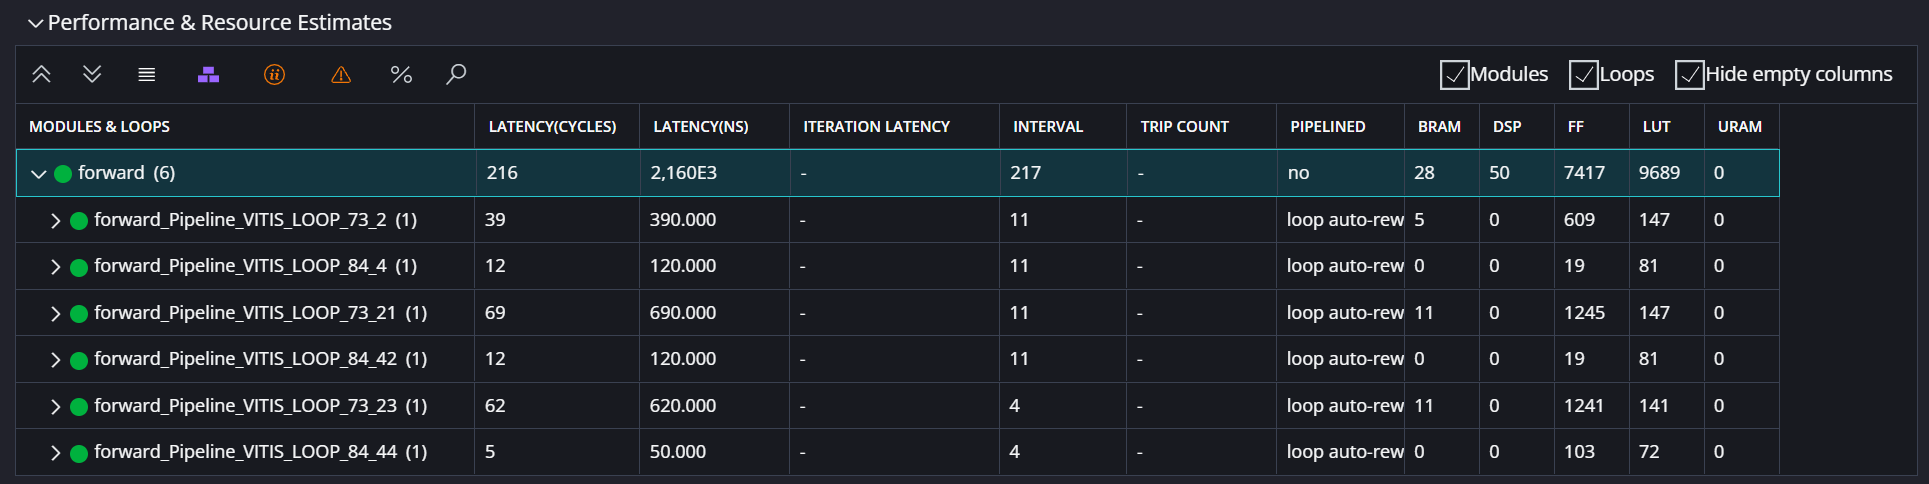
\includegraphics[width=1\textwidth]{./assets/MLP/c-synthesis-performanceandresourceestimaes.png}
    \caption{Perfomance and Resource Estimates in the C-Synthesis Report}
    \label{fig:c-synthesis-performance-resources}
\end{figure}

From the above image, we observe that the \texttt{forward} module exhibits an overall estimated latency of 216 cycles, corresponding to an execution time of 2,160 ns under the target clock frequency of 100 MHz (10 ns per cycle). The initiation interval (II) for the main module is reported as 217 cycles, which indicates that the design could benefit from further pipelining to optimize parallel execution and reduce the interval.

Examining the resource utilization, the design employs:
\begin{itemize}
    \item \textbf{9,689 Look-Up Tables (LUTs)}, which corresponds to approximately 67.3\% of the total 14,400 LUTs available on the \texttt{xc7z007s-clg225-2}.
    \item \textbf{7,417 Flip-Flops (FFs)}, utilizing 25.7\% of the total 28,800 FFs available.
    \item \textbf{50 DSP slices}, accounting for 75.8\% of the total 66 available DSPs.
    \item \textbf{No BRAM or URAM}, which indicates that the design relies solely on external or internal registers for data storage.
\end{itemize}

The internal loops of the \texttt{forward} pass module demonstrate varied latencies, with some loops optimized using \texttt{\#pragma HLS UNROLL} and \texttt{\#pragma HLS PIPELINE}. Latencies range from 5 ns to 690 ns, with the primary loop exhibiting the highest latency (690 ns). This latency suggests potential bottlenecks in data dependencies or resource contention, which could be addressed by restructuring loops or leveraging more efficient parallelization strategies.

To further enhance performance, improvements such as increasing the use of internal memory resources (e.g., BRAM/URAM) and reducing loop dependencies are recommended. These adjustments would help lower the initiation interval and improve overall throughput, making the design more efficient for hardware acceleration.
\\\\We can also check from the report that, as expected the hardware interface corresponds to the input and output of the forward pass function, and that the utilized pragma syntax is correct and corresponds to the one we used in the code.

\begin{figure}[H]
    \centering
    \begin{minipage}{0.49\textwidth}
        \centering
        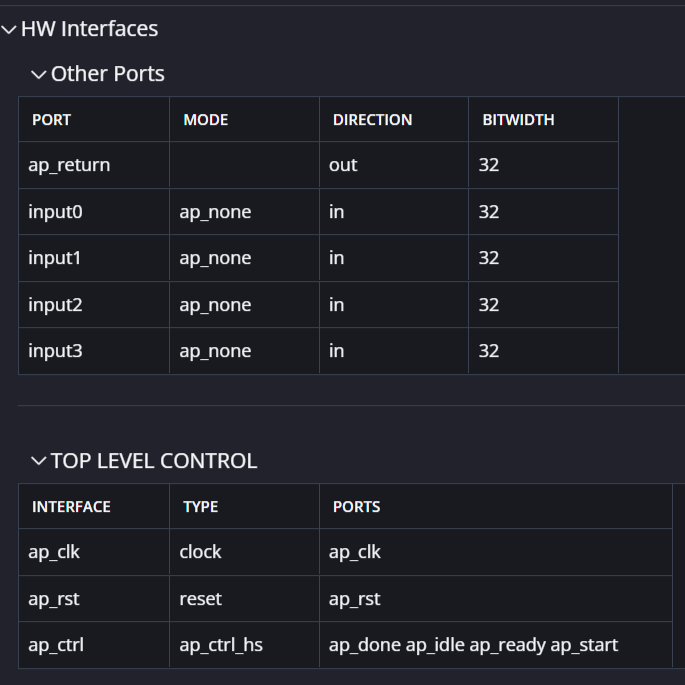
\includegraphics[width=1\textwidth]{./assets/MLP/c-synthesis-HWinterfaces.png}
        \caption{Hardware interfaces}
        \label{fig:c-synthesis-hw-interfaces}
    \end{minipage}
    \hfill
    \begin{minipage}{0.49\textwidth}
        \centering
        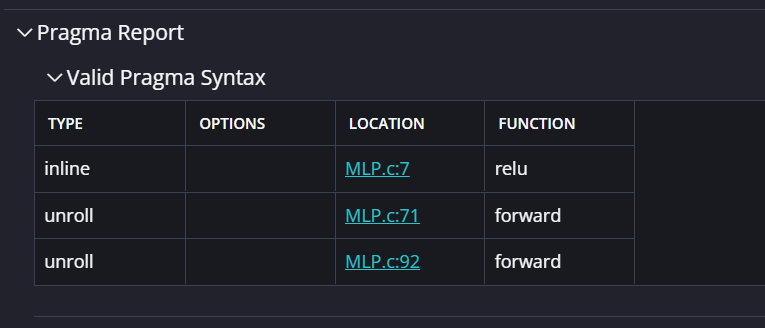
\includegraphics[width=1\textwidth]{./assets/MLP/c-synthesis-validpragmasyntax.png}
        \caption{Pragma syntax}
        \label{fig:c-synthesis-pragma-syntax}
    \end{minipage}
\end{figure}


\paragraph{C/RTL Simulation}

C-RTL cosimulation is a verification process that ensures the functional equivalence between the high-level C/C++ design and the synthesized Register-Transfer Level (RTL) code. This step is critical as it confirms that the behavior of the RTL implementation matches the original C/C++ description after synthesis. The benefits are multiple:

\begin{itemize}
    \item \textbf{Validation of Functional Correctness}: Verifies that the generated RTL implementation functions identically to the original high-level design for the same inputs.
    \item \textbf{Timing and Latency Estimates}: Provides insights into the actual timing behavior of the synthesized RTL.
    \item \textbf{Resource Utilization Check}: Highlights any discrepancies between resource usage reported during synthesis and actual utilization in hardware.
\end{itemize}

\subparagraph{How It Works}
\begin{enumerate}
    \item \textbf{Input Stimuli}: A testbench written in C/C++ is used to provide input data to both the high-level C/C++ design and the RTL design.
    \item \textbf{Output Comparison}: The outputs from the high-level simulation and the RTL simulation are compared.
    \item \textbf{Reports}: Any mismatches or timing violations are reported for debugging purposes.
\end{enumerate}


\begin{figure}[H]
    \centering
    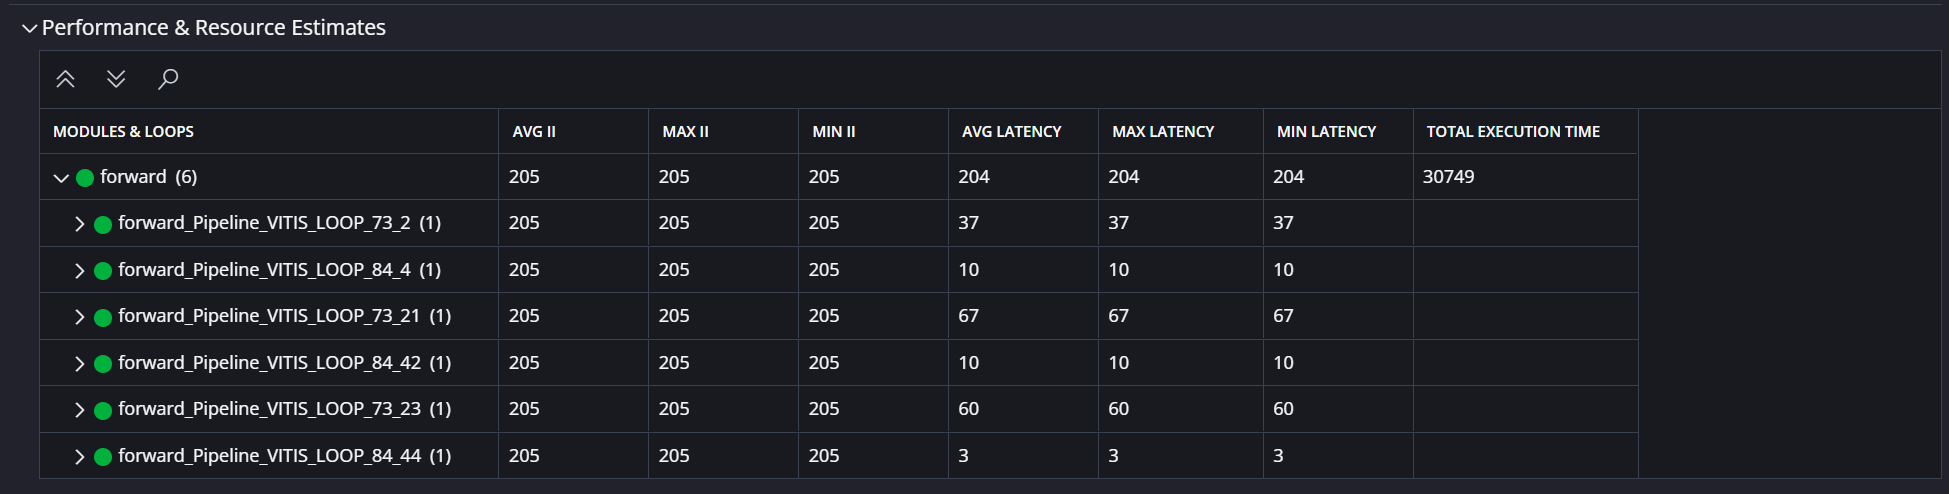
\includegraphics[width=1\textwidth]{./assets/MLP/c-rtl-cosimulation.png}
    \caption{C/RTL Cosimulation Report - Performance and resource estimates}
    \label{fig:C-RTL-cosimulation}
\end{figure}


\subsubsection{Analysis of Results}

The analysis of the results from the C/RTL co-simulation and synthesis reports highlights several key observations and metrics:

\begin{itemize}
    \item \textbf{Initiation Interval (II):} The initiation interval across all loops in the design remains constant at \textbf{205 cycles}. This uniform II suggests a consistent level of pipelining efficiency across the design. However, it also indicates that certain dependencies or resource constraints may limit further reduction of the II.

    \item \textbf{Loop Latencies:} The latencies for individual loops vary significantly:
    \begin{itemize}
        \item The loop labeled \texttt{forward\_Pipeline\_VITIS\_LOOP\_73\_2} exhibits an average latency of \textbf{37 cycles}, which aligns with expectations for its complexity.
        \item Other loops, such as \texttt{forward\_Pipeline\_VITIS\_LOOP\_84\_44}, achieve minimal latencies of just \textbf{3 cycles}, indicating highly efficient implementation.
    \end{itemize}
    The overall latency of the forward pass main module is \textbf{204 cycles}, which matches the expected values from the high-level design.

    \item \textbf{Total Execution Time:} The total execution time for the forward pass is reported as 30,749 ns. This result reflects the aggregated runtime of all components and their interactions.

    \item \textbf{Pipeline Observations:} While the loops in the forward pass are pipelined, the relatively high initiation interval (205 cycles) suggests potential bottlenecks. These could stem from data dependencies or limited resource availability, particularly in critical paths of the design.

    \item \textbf{Resource Utilization:} 
    \begin{itemize}
        \item The design effectively utilizes available DSPs, LUTs, and Flip-Flops, as previously described.
        \item However, no usage of BRAM or URAM is reported. Leveraging these resources could reduce dependency on external memory and improve performance in memory-intensive operations.
    \end{itemize}
\end{itemize}

\paragraph{Observations and Suggestions}
The results confirm that the design is functional and performs as expected. However, several areas for improvement are identified:
\begin{enumerate}
    \item \textbf{Reducing II:} Efforts should be directed towards decreasing the initiation interval by addressing resource contention and loop dependencies. Techniques such as loop unrolling or splitting could be beneficial.
    \item \textbf{Memory Utilization:} Introducing BRAM or URAM for intermediate data storage can minimize external memory accesses and improve throughput.
    \item \textbf{Optimization of Critical Loops:} High-latency loops should be reviewed and restructured to enhance parallelism, potentially improving the overall execution time.
\end{enumerate}

By implementing these optimizations, the design could achieve higher efficiency and better alignment with the hardware capabilities of the target FPGA device.

\paragraph{Packaging}
Regarding the \textit{Package} section, there is  not much to be said, since the Vitis IDE doesn't provide a report for this stage. However, we can still infer that the packaging process was successful, as the design was ready for the final implementation stage.

\paragraph{Implementation}

Here in this section we can mainly analyze the \textit{RTL synthesis} and the \textit{Place and Route} stages: the first provides a detailed report on the synthesis of the design into Register-Transfer Level (RTL) code, while the latter focuses on the physical implementation of the design on the FPGA.
Regarding the \textit{RTL synthesis}, the report provides insights into the resource utilization, timing constraints, and design hierarchy. The metrics include the number of Look-Up Tables (LUTs), Flip-Flops (FFs), and Digital Signal Processors (DSPs) used, as well as the critical path delay and maximum frequency. These metrics are crucial for assessing the design's efficiency and performance, guiding further optimization efforts.
\\\\ From the \textit{Implementation Report} results, the following observations can be made:

\begin{itemize}
    \item \textbf{Resource Utilization:} The design consumes a total of 4,438 LUTs, 5,332 FFs, 50 DSP blocks, 11 BRAMs, and 104 SRLs. Notably, no URAM, latches, or slices are utilized. This indicates an efficient use of FPGA resources without exceeding critical limits.
    \item \textbf{Timing Constraints:}
    The required clock period for the design is set to 10.000 ns, corresponding to a target clock frequency of 100 MHz. During the synthesis phase, the achieved clock period is reported as 6.872 ns, which exceeds the performance requirements and indicates that the synthesized design meets the desired constraints. However, after implementation, the achieved clock period is reported as 7.860 ns. While this is slightly higher than the synthesized value, it still satisfies the required 10.000 ns clock period. 
    
    The increase in the clock period from synthesis to implementation can be attributed to additional routing delays and resource constraints introduced during placement and routing. These results confirm that the design meets the required timing constraints post-implementation while providing a buffer for further optimizations if needed.
    
\end{itemize}

\subsubsection{Fail Fast Analysis}

The Fail Fast analysis is a preliminary verification step designed to ensure that the design adheres to fundamental guidelines before proceeding to computationally intensive stages such as placement and routing. This stage evaluates key aspects of the design, including resource utilization and timing constraints, to identify potential bottlenecks early in the development process.

The following columns are analyzed:

\begin{itemize}
    \item \textbf{Criteria:} Key aspects of the design, such as LUT usage, FD (Flip-Flop Density), and DFP (Dynamic Floating-Point operations), are monitored to ensure they fall within acceptable thresholds.
    \item \textbf{Guideline:} Defines a reference threshold for each criterion to guide the design toward optimal FPGA resource usage and performance.
    \item \textbf{Actual:} Displays the measured values of each criterion after the analysis of the current design.
    \item \textbf{State:} Indicates the compliance status of each criterion, with possible values:
    \begin{itemize}
        \item \textbf{OK:} The criterion satisfies the guideline and requires no action.
        \item \textbf{WARNING:} The criterion approaches the threshold, suggesting caution.
        \item \textbf{FAIL:} The criterion exceeds the guideline, necessitating immediate attention.
    \end{itemize}
\end{itemize}

\paragraph{Criteria Evaluated:}
\begin{itemize}
    \item \textbf{LUT Usage:} Monitors the utilization of Look-Up Tables, ensuring that logic mapping remains within device capacity.
    \item \textbf{Flip-Flop Density:} Assesses the distribution of flip-flops to avoid routing congestion.
    \item \textbf{DSP Allocation:} Evaluates the usage of DSP slices for arithmetic operations, critical for neural network implementations.
    \item \textbf{Timing Constraints:} Verifies whether the design meets the required clock period and ensures no timing violations.
\end{itemize}

\paragraph{Results:}
The analysis revealed that all criteria were marked as \texttt{OK}, indicating that the design complies with resource and timing guidelines. A summary of the key metrics is shown in Table~\ref{tab:failfast-results}.

\begin{table}[h]
    \centering
    \begin{tabular}{|c|c|c|c|}
        \hline
        \textbf{Criteria} & \textbf{Threshold} & \textbf{Actual} & \textbf{Status} \\
        \hline
        LUT Usage         & 14,400             & 3,738           & OK \\
        Flip-Flop Usage   & 28,800             & 5,364           & OK \\
        DSP Allocation    & 66                 & 50              & OK \\
        BRAM Usage        & 50                 & 11              & OK \\
        \hline
    \end{tabular}
    \caption{Fail Fast Analysis Results}
    \label{tab:failfast-results}
\end{table}

\paragraph{Observations and Recommendations:}
\begin{enumerate}
    \item \textbf{Resource Utilization:} While all resources are within acceptable thresholds, DSP allocation is relatively high at 75.8\%. Future optimizations could focus on reducing DSP dependency by leveraging LUTs for simpler arithmetic operations.
    \item \textbf{Timing Constraints:} The achieved clock period of 7.860 ns provides sufficient margin against the required 10.000 ns, demonstrating robust timing compliance.
    \item \textbf{Critical Loops:} If further optimizations are required, consider reviewing high-latency loops to improve pipeline efficiency and reduce initiation intervals.
\end{enumerate}

The combination of the \textit{Implementation Report} and \textit{Fail Fast} analysis highlights the robustness of the design, ensuring efficient resource utilization and adherence to timing requirements while avoiding potential pitfalls early in the development process.




\begin{figure}[H]
    \centering
    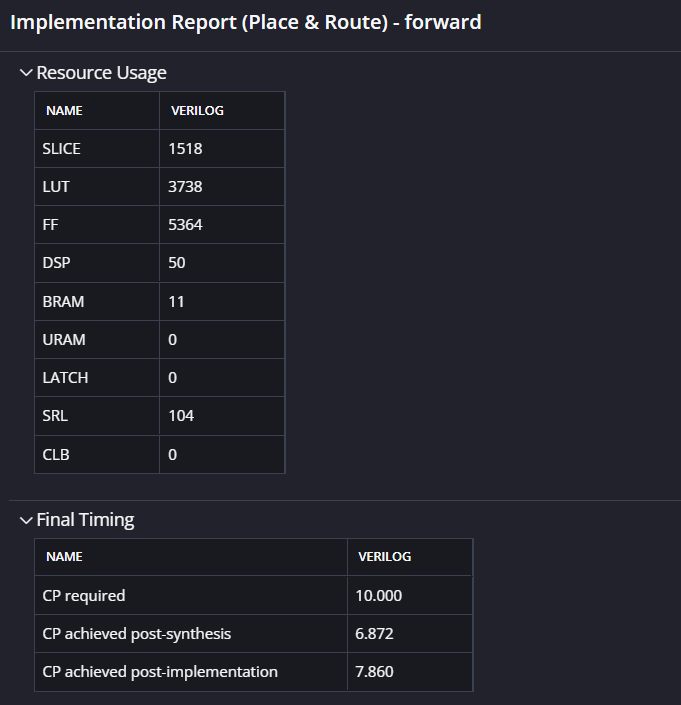
\includegraphics[width=0.5\textwidth]{./assets/MLP/implementation-resourceusagefinaltiming.png}
    \caption{Resource Usage and Final Timing Report in the RTL Synthesis}
    \label{fig:rtl-synthesis}
\end{figure}




\begin{figure}[H]
    \centering
    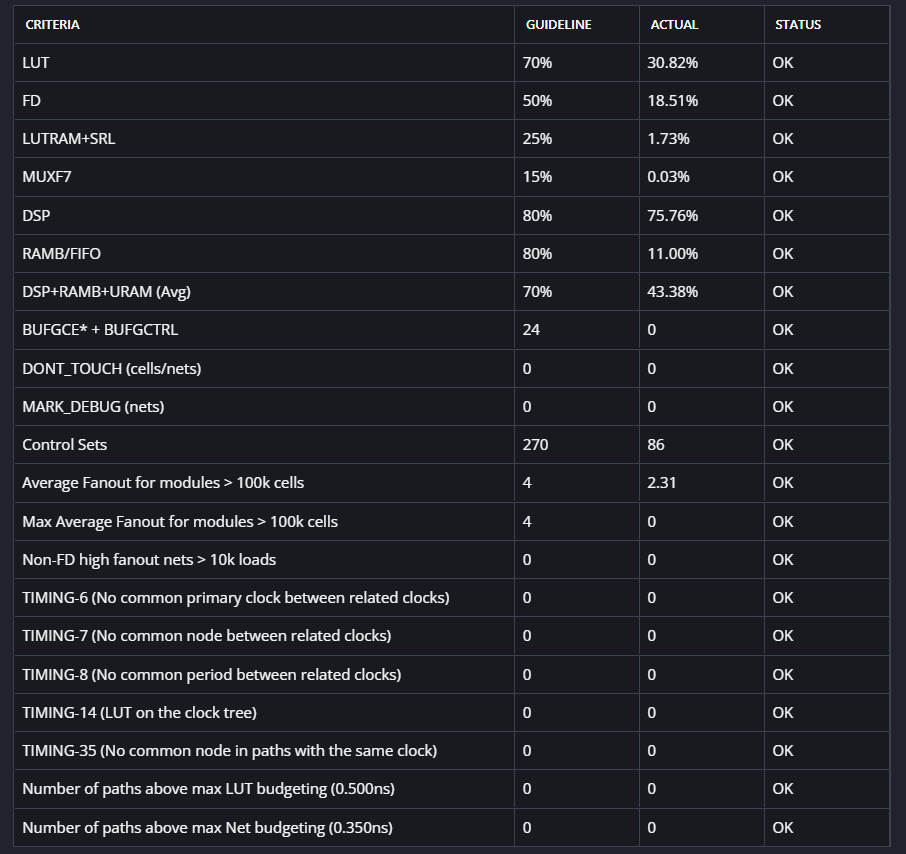
\includegraphics[width=0.5\textwidth]{./assets/MLP/implementation-failfast.png}
    \caption{Fail Fast Report in the RTL Synthesis}
    \label{fig:fail-fast}
\end{figure}

\newpage


\section{Convolutional Neural Network (CNN)}
Convolutional Neural Networks (CNNs) are a class of deep learning models specifically designed to process grid-like data, such as images. Their ability to automatically learn spatial hierarchies of features makes them highly effective for image classification tasks. In this implementation, a simple yet efficient CNN is designed and trained to classify handwritten digits from the famuos MNIST dataset, with the aim of achieving high accuracy while remaining compatible with hardware synthesis constraints. So the ConvNet forward pass was implemented in a similar manner to the MLP, with the main difference being the convolution and pooling operations.


\subsection{Dataset}
The CNN was trained on the MNIST dataset, a widely used benchmark for handwritten digit classification tasks. The dataset consists of 70,000 grayscale images of digits (0,1,2,3,4,5,6,7,8,9), each with a resolution of $28 \times 28$ pixels. The dataset was split into two subsets, with 70\% used as the training set and 30\% as the validation set, resulting in the following distribution:

\begin{itemize}
    \item Training set: 42,000 samples.
    \item Validation set: 18,000 samples.
    \item Test set: 10,000 samples for evaluating the model's performance.
\end{itemize}

The dataset was preprocessed using normalization to scale pixel values to the range $[-1, 1]$, this normalization centers the pixel values around 0 and scales them to have a standard deviation of 1, which can often help with model training and convergence.


\subsection{PyTorch Model}

\subsubsection{Model Architecture}
The ConvNet is designed to be as simple as possible, ensuring efficiency and compatibility with hardware synthesis using Vitis HLS. The structure includes the following layers:
\begin{itemize}
    \item \textbf{Convolutional Layer:} A single convolutional layer with 3 filters, each of size $3 \times 3$, stride $1$, and padding $1$. This layer increases feature representation by extracting local patterns from the input images.
    \item \textbf{ReLU Activation:} Applied after the convolutional layer to introduce non-linearity into the model.
    \item \textbf{Pooling Layer:} A max-pooling layer with a kernel size of $2 \times 2$ and a stride of $2$, reducing the spatial dimensions of the feature map by half.
    \item \textbf{Fully Connected Layer:} It takes as input the flattened feature map from the convolutional and pooling layers. As output 10 neurons representing the 10 digit classes (0–9). This layer does not apply an activation function, as it is followed by the softmax during training or inference.
\end{itemize}

The forward pass through the network is as follows:
\begin{enumerate}
    \item Apply the convolutional layer to the input image, followed by the ReLU activation function.
    \item Perform max-pooling on the resulting feature map.
    \item Flatten the feature map into a one-dimensional vector.
    \item Pass the flattened vector through the fully connected layer to produce class probabilities.
\end{enumerate}

The simplicity of this architecture ensures compatibility with hardware synthesis while maintaining high accuracy for digit classification tasks.\\

The model was defined as follows, using the \textit{PyTorch} library:

\begin{lstlisting}[language=Python]
# Define the CNN model
class ConvNet(nn.Module):
    def __init__(self):
        super(ConvNet, self).__init__()
        # Input: x = [1, 28, 28]
        self.conv1 = nn.Conv2d(1, 3, kernel_size=3, stride=1, padding=1)  
        # Convolutional Layer: Output: x = [3, 28, 28]
        # Formula: (W - F + 2P) / S + 1
        self.pool = nn.MaxPool2d(kernel_size=2, stride=2)  
        # Pooling Layer: Output: x = [3, 14, 14]
        # Formula: (W - F) / S + 1
        self.fc1 = nn.Linear(3 * 14 * 14, 10)  
        # Fully Connected Layer: Flatten the output to match 10 classes

    def forward(self, x):
        x = torch.relu(self.conv1(x))  # Apply ReLU after convolution
        x = self.pool(x)              # Apply max pooling
        x = x.view(x.size(0), -1)     # Flatten the tensor
        x = self.fc1(x)               # Fully connected layer
        return x
\end{lstlisting}



\subsubsection{Model Training}
The training process for the Convolutional Neural Network (CNN) was performed using the \textit{PyTorch} library. The objective was to minimize the cross-entropy loss, a suitable loss function for multi-class classification problems. The training configuration was as follows:
\begin{itemize}
    \item \textbf{Loss Function:} CrossEntropyLoss.
    \item \textbf{Optimizer:} Adam optimizer with a learning rate of 0.001.
    \item \textbf{Batch Size:} 64.
    \item \textbf{Epochs:} 100.
\end{itemize}

\begin{lstlisting}[language=Python]
# initialize network, loss function and optimizer
model = ConvNet().to(device)
criterion = nn.CrossEntropyLoss()
optimizer = optim.Adam(model.parameters(), lr=learning_rate)
\end{lstlisting}

The training procedure involved the following steps:
\begin{enumerate}
    \item The input images were passed through the CNN in a forward pass to compute the predicted class probabilities.
    \item The CrossEntropyLoss function was used to calculate the loss between the predicted and actual class labels.
    \item Backpropagation was performed to compute the gradients of the loss with respect to the model parameters.
    \item The Adam optimizer was used to update the parameters using the calculated gradients.
\end{enumerate}

After each epoch, the model was evaluated on the validation set to monitor its performance. The accuracy and loss for both training and validation sets were recorded for further analysis.

\clearpage
\begin{table}[htbp]
    \centering
    \caption{Training and Validation Results at Selected Epochs}
    \label{tab:training-results}
    \renewcommand{\arraystretch}{1.2} % Increase row spacing
    \begin{tabular}{|c|c|c|c|c|}
    \hline
    \textbf{Epoch} & \textbf{Train Loss} & \textbf{Train Accuracy (\%)} & \textbf{Val Loss} & \textbf{Val Accuracy (\%)} \\ \hline
    10             & 0.1194             & 96.49                        & 0.1360            & 96.03                       \\ \hline
    20             & 0.0907             & 97.30                        & 0.1232            & 96.38                       \\ \hline
    30             & 0.0735             & 97.74                        & 0.1130            & 96.77                       \\ \hline
    40             & 0.0636             & 98.03                        & 0.1122            & 96.79                       \\ \hline
    50             & 0.0571             & 98.27                        & 0.1147            & 96.75                       \\ \hline
    60             & 0.0521             & 98.34                        & 0.1147            & 96.88                       \\ \hline
    70             & 0.0491             & 98.39                        & 0.1259            & 96.73                       \\ \hline
    80             & 0.0459             & 98.53                        & 0.1285            & 96.69                       \\ \hline
    90             & 0.0439             & 98.55                        & 0.1342            & 96.61                       \\ \hline
    100            & 0.0411             & 98.71                        & 0.1325            & 96.76                       \\ \hline
    \end{tabular}
\end{table}
    

The final test performance was as follows:
\begin{itemize}
    \item \textbf{Test Loss:} 0.1260
    \item \textbf{Test Accuracy:} 97.06\%
\end{itemize}


The following Python code snippet shows the main training loop:
\begin{lstlisting}[language=Python]
# Training loop
for epoch in range(NUM_EPOCHS):
    model.train()
    train_loss = 0.0
    train_correct = 0
    train_total = 0

    for images, labels in train_loader:
        images, labels = images.to(device), labels.to(device)

        optimizer.zero_grad()
        outputs = model(images)
        loss = criterion(outputs, labels)
        loss.backward()
        optimizer.step()

        train_loss += loss.item()
        _, predicted = outputs.max(1)
        train_total += labels.size(0)
        train_correct += predicted.eq(labels).sum().item()

    train_accuracy = 100. * train_correct / train_total

    # Validation phase
    model.eval()
    val_loss = 0.0
    val_correct = 0
    val_total = 0

    with torch.no_grad():  # Disable gradient calculations
        for images, labels in val_loader:
            images, labels = images.to(device), labels.to(device)

            outputs = model(images)
            loss = criterion(outputs, labels)

            val_loss += loss.item()
            _, predicted = outputs.max(1)
            val_total += labels.size(0)
            val_correct += predicted.eq(labels).sum().item()

    val_accuracy = 100. * val_correct / val_total

    if (epoch + 1) % 10 == 0:
        print(f"Epoch [{epoch + 1}/{NUM_EPOCHS}], "
              f"Train Loss: {train_loss / len(train_loader):.4f}, Train Acc: {train_accuracy:.2f}%, "
              f"Val Loss: {val_loss / len(val_loader):.4f}, Val Acc: {val_accuracy:.2f}%")
\end{lstlisting}



\subsubsection{Exporting Parameters}
To facilitate hardware implementation, the trained parameters (weights and biases) of the CNN model were exported to a structured format. This process allows the model to be reimplemented in a different environment, such as a C-based hardware description.

The following Python code was used to extract and store the parameters:

\begin{lstlisting}[language=Python]
weights = {}
total_params = 0
for name, param in model.to("cpu").named_parameters():
    weights[name] = param.detach().numpy()
    layer_params = param.numel()
    total_params += layer_params
    print(f"{name}: {param.shape}, Total Parameters: {layer_params}")

print(f"Total Parameters in the model: {total_params}")
\end{lstlisting}

This process ensures the trained model can be effectively utilized in hardware environments, preserving its performance and structure.


\subsection{C Implementation}
The implementation of the Convolutional Neural Network (CNN) model in C is divided into three main files:

\begin{itemize}
    \item \texttt{ConvNet.h}: This header file defines the data structures and constants used in the implementation, including the convolutional and fully connected layers, and the overall network structure.
    \item \texttt{ConvNet.c}: This file contains the implementation of the CNN's functionality, including the forward pass and activation functions, along with predefined weights and biases.
    \item \texttt{testbench.c}: This file serves as a testbench to verify the network's functionality. It includes functions for reading input data, executing the forward pass, and evaluating the model's output against the expected results.
\end{itemize}

This modular approach ensures clarity and separation of concerns, allowing for easy modification and testing of individual components. The details of each file are described in the following subsections.


\subsubsection{CNN Structure}
The Convolutional Neural Network (CNN) structure is implemented in C to match the architecture defined in the PyTorch model. It consists of the following components:

\begin{itemize}
    \item \textbf{Convolutional Layer:} This layer performs the convolution operation by sliding a set of filters (or kernels) over the input image to extract spatial features. The implementation uses nested loops to apply the filters, taking into account padding and stride.
    \item \textbf{ReLU Activation:} The Rectified Linear Unit (ReLU) activation function is applied after the convolutional operation to introduce non-linearity. The ReLU function replaces negative values in the feature map with zeros.
    \item \textbf{Pooling Layer:} A max-pooling operation reduces the spatial dimensions of the feature map by selecting the maximum value within a kernel-sized region. This layer helps to downsample the feature map and make the model more robust to small spatial variations.
    \item \textbf{Fully Connected Layer:} The fully connected layer takes the flattened output from the pooling layer as input and maps it to the output classes. This is achieved by performing a linear transformation using the preloaded weights and biases.
\end{itemize}

The CNN structure is defined in the header file \texttt{ConvNet.h}, which outlines the data structures and constants used for the network. The file also declares the \texttt{forward} function responsible for executing the network. Here the ConvNet structure:

\begin{lstlisting}[language=C]
// Structure to represent a convolutional layer
typedef struct {
    float weights[CONV1_OUTPUT_CHANNELS][INPUT_CHANNELS][3][3]; // Filters of the convolutional layer 
    float biases[CONV1_OUTPUT_CHANNELS];                        // Biases for the filters
} ConvLayer;

// Structure to represent a fully connected layer
typedef struct {
    float weights[NUM_CLASSES][FC1_INPUT_SIZE]; // Weights of the fully connected layer
    float biases[NUM_CLASSES];                 // Biases of the fully connected layer
} FullyConnectedLayer;

// General structure of the network
typedef struct {
    ConvLayer conv1;               // First convolutional layer
    FullyConnectedLayer fc1;       // Fully connected layer
} ConvNet;
\end{lstlisting}

\subsubsection{Forward Pass}
The forward pass function propagates an input image through the Convolutional Neural Network (CNN) to generate the class probabilities as output. This involves executing the convolution, activation, pooling, and fully connected layers sequentially.

The following C code implements the forward pass:

\begin{lstlisting}[language=C]
// Forward pass function
int forward(float input[INPUT_HEIGHT][INPUT_WIDTH][INPUT_CHANNELS], float output[NUM_CLASSES]) {

    // Convolutional layer output buffer
    float conv_output[CONV1_OUTPUT_CHANNELS][INPUT_HEIGHT][INPUT_WIDTH];
    #pragma HLS ARRAY_PARTITION variable=conv_output complete dim=1

    // Convolutional layer operation
    for (int oc = 0; oc < CONV1_OUTPUT_CHANNELS; oc++) {
        for (int h = 0; h < INPUT_HEIGHT; h++) {
            for (int w = 0; w < INPUT_WIDTH; w++) {
                float sum = convnet.conv1.biases[oc];
                for (int ic = 0; ic < INPUT_CHANNELS; ic++) {
                    for (int kh = 0; kh < 3; kh++) {
                        for (int kw = 0; kw < 3; kw++) {
                            int ih = h + kh - 1;
                            int iw = w + kw - 1;
                            if (ih >= 0 && iw >= 0 && ih < INPUT_HEIGHT && iw < INPUT_WIDTH) {
                                sum += input[ih][iw][ic] * convnet.conv1.weights[oc][ic][kh][kw];
                            }
                        }
                    }
                }
                conv_output[oc][h][w] = reLu(sum);
            }
        }
    }

    // MaxPooling layer output buffer
    float pool_output[CONV1_OUTPUT_CHANNELS][INPUT_HEIGHT / POOL_SIZE][INPUT_WIDTH / POOL_SIZE];
    #pragma HLS ARRAY_PARTITION variable=pool_output complete dim=1

    // MaxPooling operation
    for (int oc = 0; oc < CONV1_OUTPUT_CHANNELS; oc++) {
        for (int h = 0; h < INPUT_HEIGHT / POOL_SIZE; h++) {
            for (int w = 0; w < INPUT_WIDTH / POOL_SIZE; w++) {
                float max_val = -1e9;
                for (int ph = 0; ph < POOL_SIZE; ph++) {
                    for (int pw = 0; pw < POOL_SIZE; pw++) {
                        int ih = h * POOL_SIZE + ph;
                        int iw = w * POOL_SIZE + pw;
                        if (ih < INPUT_HEIGHT && iw < INPUT_WIDTH) {
                            max_val = fmaxf(max_val, conv_output[oc][ih][iw]);
                        }
                    }
                }
                pool_output[oc][h][w] = max_val;
            }
        }
    }

    // Fully connected layer input buffer
    float fc_input[FC1_INPUT_SIZE];
    #pragma HLS ARRAY_PARTITION variable=fc_input complete

    // Flatten pooling output into 1D array
    int idx = 0;
    for (int oc = 0; oc < CONV1_OUTPUT_CHANNELS; oc++) {
        for (int h = 0; h < INPUT_HEIGHT / POOL_SIZE; h++) {
            for (int w = 0; w < INPUT_WIDTH / POOL_SIZE; w++) {
                fc_input[idx++] = pool_output[oc][h][w];
            }
        }
    }

    // Fully connected layer computation
    for (int o = 0; o < NUM_CLASSES; o++) {
        float sum = convnet.fc1.biases[o];
        for (int i = 0; i < FC1_INPUT_SIZE; i++) {
            sum += fc_input[i] * convnet.fc1.weights[o][i];
        }
        output[o] = sum;
    }

    return 0; // Success
}
\end{lstlisting}

This implementation uses \texttt{\#pragma HLS ARRAY\_PARTITION} to optimize memory access patterns, enabling efficient synthesis for hardware acceleration.
As with the MLP implementation, all weights and biases in the CNN are hardcoded and directly integrated into the \texttt{ConvNet.c} file. This approach ensures that the trained parameters from the PyTorch model are seamlessly incorporated into the C-based implementation for efficient execution.


\subsubsection{Testbench}
\subsubsection{Testbench}
The testbench is a critical component for validating the correctness of the CNN implementation in C. It reads input data from a file, processes it through the CNN using the \texttt{forward} function, and verifies the output against the expected label. This ensures that the implementation behaves as expected and aligns with the PyTorch model.

The testbench performs the following key tasks:
\begin{itemize}
    \item \textbf{Input Loading}: Reads the input image and its corresponding label from a text file (\texttt{input\_image.txt}).
    \item \textbf{Forward Pass Execution}: Propagates the input through the CNN to compute class probabilities.
    \item \textbf{Result Validation}: Compares the predicted label with the true label and outputs the result.
\end{itemize}

The following code demonstrates the implementation of the testbench:

\begin{lstlisting}[language=C]
#include <stdio.h>
#include <stdlib.h>
#include "ConvNet.h"

#define INPUT_FILE_PATH "./input_image.txt"
#define IMAGE_SIZE (INPUT_HEIGHT * INPUT_WIDTH) // Size of the input image

void read_input_image(const char *file_path, float input[INPUT_HEIGHT][INPUT_WIDTH][1], int *label) {
    FILE *file = fopen(file_path, "r");
    if (file == NULL) {
        perror("Failed to open input file");
        exit(EXIT_FAILURE);
    }

    // Read the label
    if (fscanf(file, "Label: %d\n", label) != 1) {
        perror("Failed to read label");
        fclose(file);
        exit(EXIT_FAILURE);
    }

    // Read the image values
    for (int h = 0; h < INPUT_HEIGHT; h++) {
        char c;
        while ((c = fgetc(file)) != EOF && (c == ' ' || c == '\n')); // Skip spaces and newlines
        if (c != '{') {
            perror("Failed to read opening brace");
            fclose(file);
            exit(EXIT_FAILURE);
        }

        for (int w = 0; w < INPUT_WIDTH; w++) {
            if (fscanf(file, "%f", &input[h][w][0]) != 1) {
                printf("Failed to read image value at (%d, %d)\n", h, w);
                fclose(file);
                exit(EXIT_FAILURE);
            }

            if (w < INPUT_WIDTH - 1) {
                if (fscanf(file, ",") != 0) {
                    perror("Failed to read comma between values");
                    fclose(file);
                    exit(EXIT_FAILURE);
                }
            }
        }

        while ((c = fgetc(file)) != EOF && (c == ' ' || c == '\n' || c == ',')); // Skip spaces and commas
        if (c != '}') {
            perror("Failed to read closing brace");
            fclose(file);
            exit(EXIT_FAILURE);
        }

        if (h < INPUT_HEIGHT - 1) {
            if (fscanf(file, ",") != 0) {
                perror("Failed to read comma between rows");
                fclose(file);
                exit(EXIT_FAILURE);
            }
        }
    }

    fclose(file);
}

int main() {
    float input[INPUT_HEIGHT][INPUT_WIDTH][INPUT_CHANNELS];
    float output[NUM_CLASSES];
    int label;

    read_input_image(INPUT_FILE_PATH, input, &label);

    int results = forward(input, output);

    if (results != 0) {
        printf("Error during forward pass\n");
        return 1;
    }

    printf("Predicted output:\n");
    for (int i = 0; i < NUM_CLASSES; i++) {
        printf("Class %d: %f\n", i, output[i]);
    }

    float max_prob = output[0];
    int predicted_label = 0;

    for (int i = 1; i < NUM_CLASSES; i++) {
        if (output[i] > max_prob) {
            max_prob = output[i];
            predicted_label = i;
        }
    }
    printf("Predicted label: %d\n", predicted_label);
    printf("True label: %d\n", label);

    return 0;
}
\end{lstlisting}

The testbench reads a structured text file containing the input image and its label. It processes the input through the CNN, identifies the predicted label, and compares it with the true label to validate the implementation's correctness.


\subsection{Results}
Text text text


\end{document}


